\chapter{Conclusion}\label{chapter:conclusion}

%Summarize thesis
This thesis used 126 $\textit{fb}^{-1}$ of data from run 2 of ATLAS
    to perform a search of the \hhproc process decaying to 4 bottom quarks,
    in order to better constrain the \kl and \kvv Higgs self-coupling constants.
The analysis made extensive use of the b-jet trigger system to identify this final state,
    alongside a b-jet pairing algorithm capable of accurately reconstructing the di-Higgs system.
An efficient selection algorithm was also employed to remove a majority of background events,
    though a sizable background still remained.
This fully hadronic final-state background was estimated using a sophisticated data-driven approach,
    which takes advantage of machine-learning algorithms specifically designed around the VBF environment.
The di-Higgs signal itself was then modeled using six Monte-Carlo simulations.
These six models were extended across the entirety of the possible \kvv/\kl/\kvv coupling parameter space
    through a linear combination technique
    which operated by reverse-engineering the fundamental QFT cross-section equation for the HH process.
Although this method initially met with severe instabilities in its modeling performance,
    I was able to derive a novel optimization procedure able to specify
    the exact Monte-Carlo simulation needed to stabilize the combination.
This additional MC sample was then used to provide an accurate hypothesis description across
    the three-dimensional \kvv/\kl/\kv parameter space,
    and so establish exclusion limits across these coupling values. 

%signal
Though the di-Higgs process itself is still too elusive for discovery with the amount of data collected so far,
    significantly tighter constraints can be placed on the \kvv and \kl coupling constants.
Indeed, for the first time constraints have been placed on the full
    3D coupling space observable via the VBF production mode of the di-Higgs process.
Courtesy of the MC sample linear combination technique,
    \kl has been constrained to between -19.5 and 23.0 for all values of \kvv with a fixed \kv=1,
    and between -10.1 and 13.3 for $\kvv=\kv=1$.
Likewise, the extrema of \kvv have been established between -0.8 and 2.8
    if \kl is permitted to fluctuate beyond its SM value while \kv is fixed to 1.
The most noteworthy results of this thesis however, is that for $\kl=\kv=1$,
    the value of \kvv can be excluded to a confidence of 95\% outside the range of $0.1 < \kvv < 2.0$.
This marks the tightest published constraints to date, improving over the latest results from CMS
    of $-0.1 < \kvv < 2.2$\cite{cms_results}.
%This leaves only one of two options, both of which are fascinating in their own ways.
%Either \kl is equal to its SM-predicted value of 1,
%    in which case \kvv must be non-zero and the \HHVV process should exist with a CL of 95\%.
%This would be the first
%    [TODO is it? Seriously I need to look at some of the past papers (and check stuff from CMS) to see how new any of this is]
%    theoretical quartic coupling,
%    and the first evidence of a Higgs four-point interaction.
%Alternately, if \kvv does not exist ($\kvv \leq 0$), then to a CL of 95\% it must be the case
%    that \kl is \textit{greater} than its SM value, which would raise any number of even more fascinating theoretical questions.
%The conclusion of this thesis leaves an ambiguity of two possible options,
%    but either possibility is quite encouraging and lends itself to future studies.

\begin{figure}
    \centering
    \begin{subfigure}{0.48\textwidth} 
        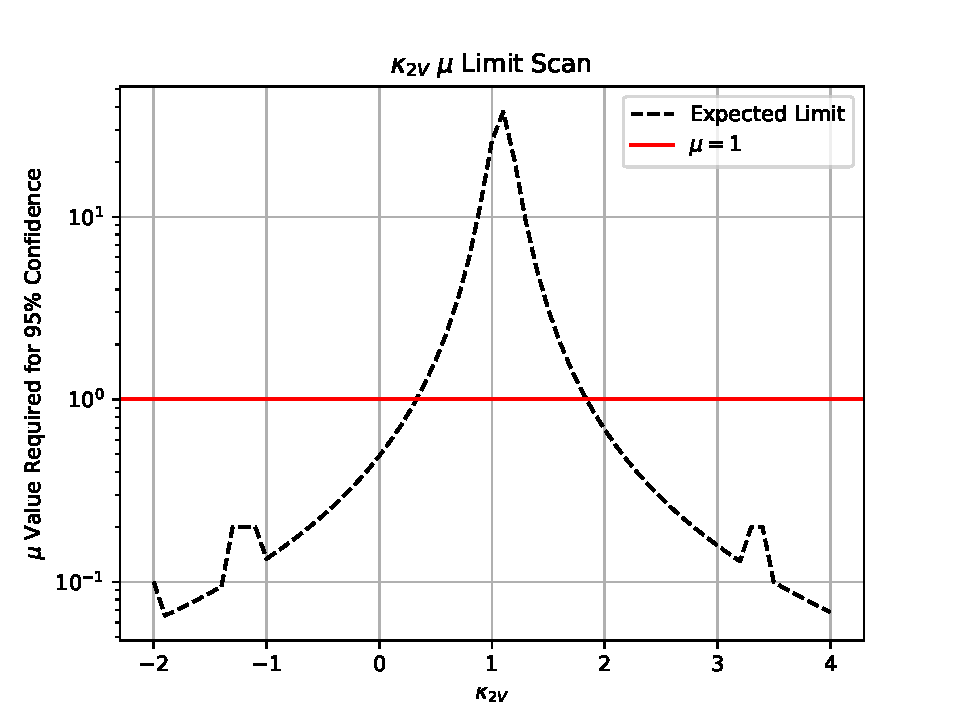
\includegraphics[width=\linewidth,height=\textheight,keepaspectratio]{conclusion/mu_limits_fast_HL-LHC_k2v}
        \caption{}%$\mu$ Scan Plot for \kvv = 1}
        \label{fig:mulimits_kvv_future}
    \end{subfigure}
    \begin{subfigure}{0.48\textwidth}
        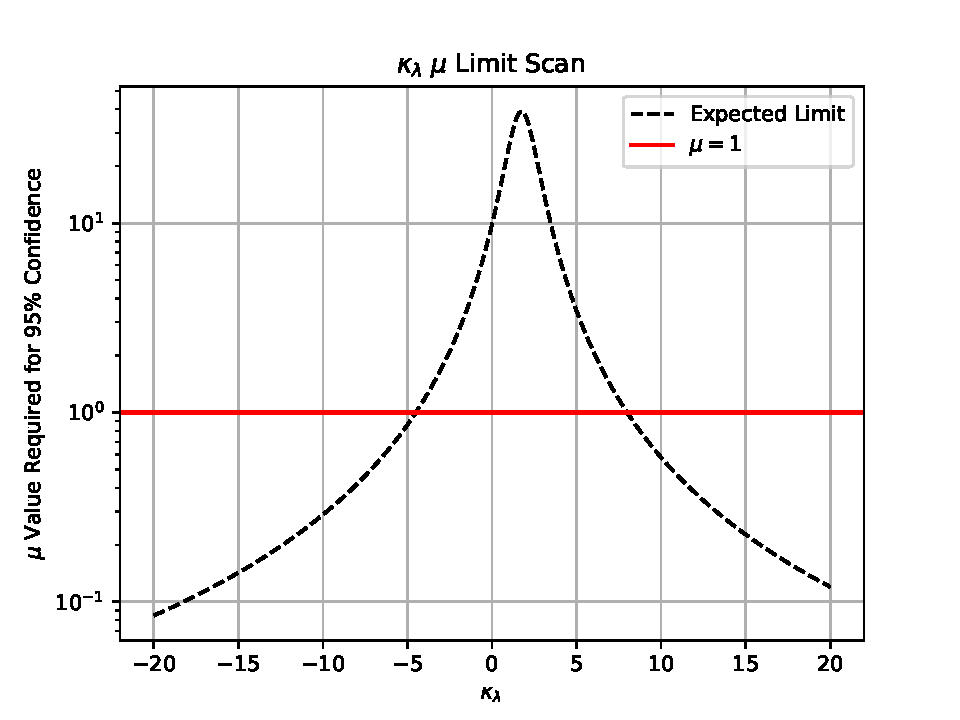
\includegraphics[width=\linewidth,height=\textheight,keepaspectratio]{conclusion/mu_limits_fast_HL-LHC_kl}
        \caption{}%$\mu$ Scan Plot for \kvv = 3}
        \label{fig:mulimits_kl_future}
    \end{subfigure}\\
    \begin{subfigure}{0.48\textwidth} 
        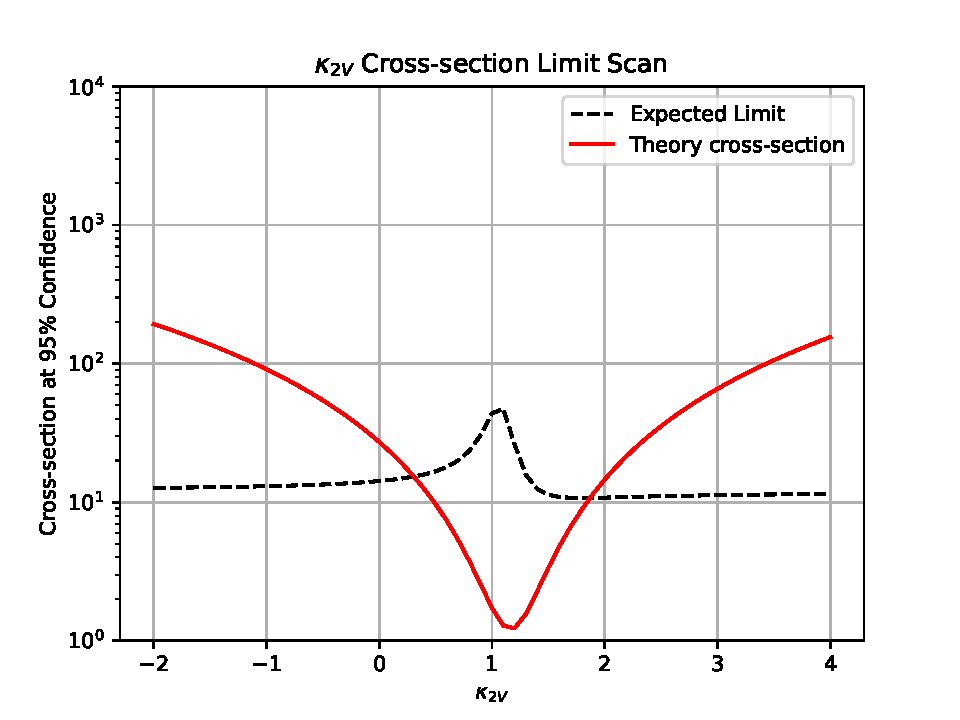
\includegraphics[width=\linewidth,height=\textheight,keepaspectratio]{conclusion/xsec_limits_fast_HL-LHC_k2v}
        \caption{}%$\mu$ Scan Plot for \kvv = 1}
        \label{fig:xseclimits_kvv_future}
    \end{subfigure}
    \begin{subfigure}{0.48\textwidth}
        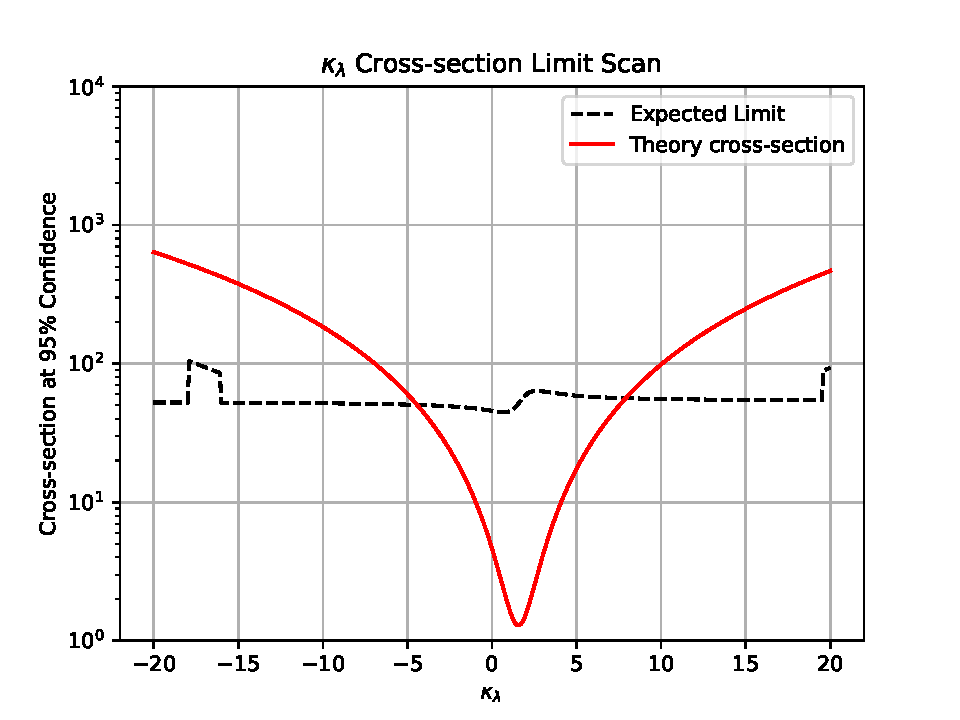
\includegraphics[width=\linewidth,height=\textheight,keepaspectratio]{conclusion/xsec_limits_fast_HL-LHC_kl}
        \caption{}%$\mu$ Scan Plot for \kvv = 3}
        \label{fig:xseclimits_kl_future}
    \end{subfigure}
    \caption{
        Figures of scans across the \kvv and \kl scaling factors
            for a hypothetical 3000 \ifb of data from the HL-LHC.
    }
    \label{fig:mu_xsec_future}
\end{figure}

%Emphasize results
Prospects for ATLAS HL-LHC are very exciting, due to the abundance of expected data.
One of the primary limiting factors in this analysis was its highly restricted sample size.
Integrated luminosity from HL-LHC is expected to reach approximately 3000 \ifb.
Rerunning the limit framework with artificially adjusted stat uncertainties produces vastly tighter constraints,
    shown in Figs. \ref{fig:mu_xsec_future} and \ref{fig:limit_slices_future}.
These projected constraints indicate vastly tighter constraints even with yields alone.
Using a full log-likelihood scan it may even be possible to detect the di-Higgs process directly.
A number of advanced techniques were pioneered in this Run 2-based analysis,
    which will surely be expanded upon in HL-LHC and beyond.
Therefore, this thesis constitutes a significant contribution to the fundamental study of the Standard Model,
    not only from the far-improved limits provided directly,
    but also by virtue of the techniques developed herein,
    which will facilitate much more efficient use of the data collected in future studies.


\begin{figure}
    \centering
    \begin{subfigure}{0.48\textwidth} 
        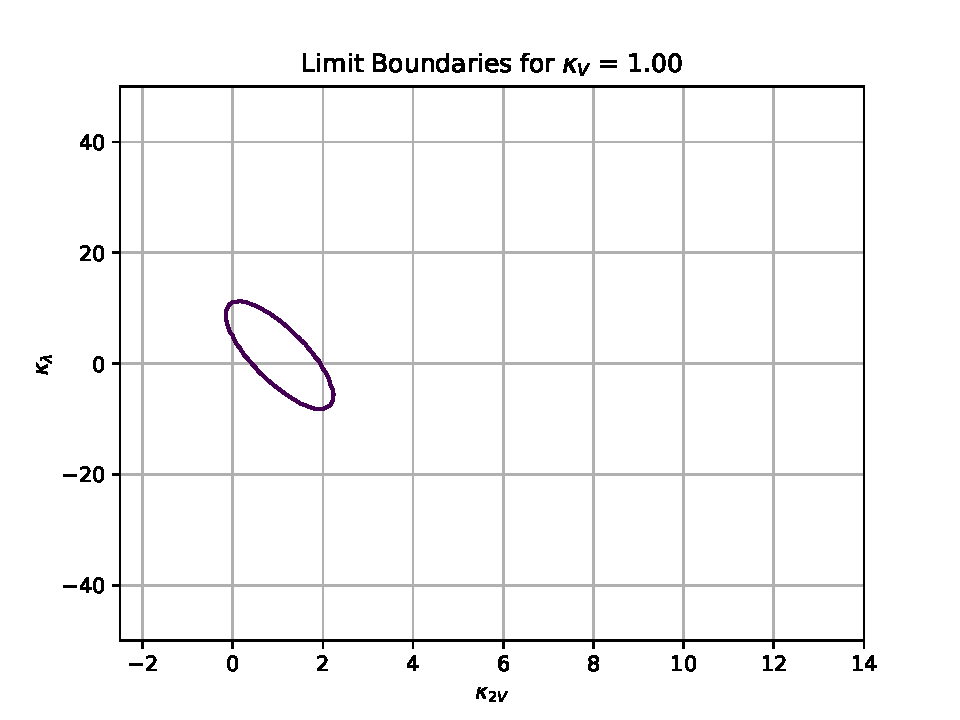
\includegraphics[width=\linewidth,height=\textheight,keepaspectratio]{conclusion/limit_slice_HL-LHC_kv_1p0}
        \caption{}
        \label{fig:limit_slice_kv_1p0_future}
    \end{subfigure}
    \begin{subfigure}{0.48\textwidth}
        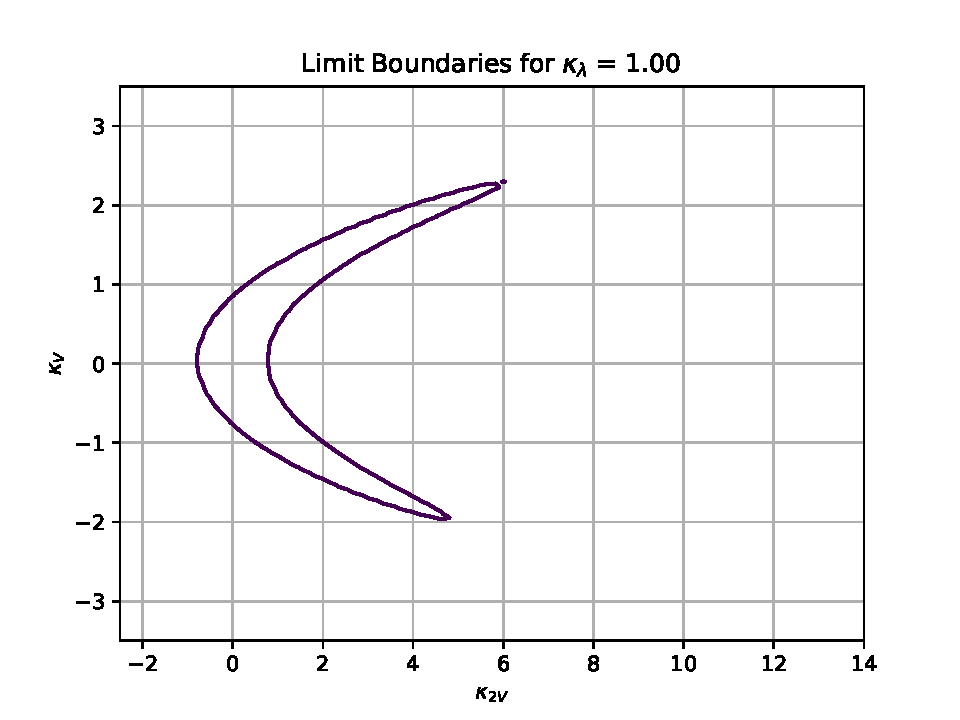
\includegraphics[width=\linewidth,height=\textheight,keepaspectratio]{conclusion/limit_slice_HL-LHC_kl_1p0}
        \caption{}
        \label{fig:limit_slice_kl_1p0_future}
    \end{subfigure}\\
    \begin{subfigure}{0.48\textwidth} 
        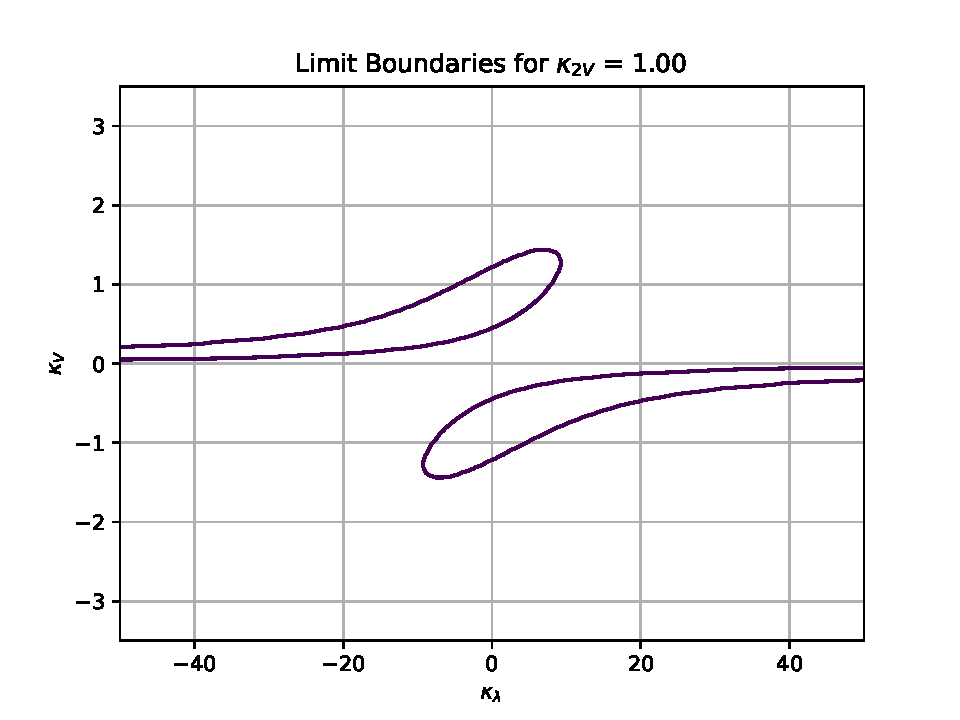
\includegraphics[width=\linewidth,height=\textheight,keepaspectratio]{conclusion/limit_slice_HL-LHC_k2v_1p0}
        \caption{}
        \label{fig:limit_slice_k2v_1p0_future}
    \end{subfigure}
    \caption{
        Two Dimensional Limit Exclusion plots for a hypothetical 3000 \ifb of data.
        The $\kappa$ scaling factors corresponding to regions outside the limit boundary
            can be excluded based on the yield of the observed data.
    }
    \label{fig:limit_slices_future}
\end{figure}


%Predict future results
